\documentclass{article}

\usepackage{fancyhdr}
\usepackage{extramarks}
\usepackage{amsmath}
\usepackage{amsthm}
\usepackage{amsfonts}
\usepackage{tikz}
\usepackage{graphicx} %插入图片的宏包
\usepackage{float} %设置图片浮动位置的宏包
\usepackage{pythonhighlight}
% \usepackage{subfigure} %插入多图时用子图显示的宏包
% \usepackage[plain]{algorithm}
% \usepackage{algpseudocode}

% \usetikzlibrary{automata,positioning}

%
% Basic Document Settings
%

\topmargin=-0.45in
\evensidemargin=0in
\oddsidemargin=0in
\textwidth=6.5in
\textheight=9.0in
\headsep=0.25in

\linespread{1.1}

\pagestyle{fancy}
\lhead{\hmwkAuthorName}
\chead{\hmwkClass\ : \hmwkTitle}
\rhead{\firstxmark}
\lfoot{\lastxmark}
\cfoot{\thepage}

\renewcommand\headrulewidth{0.4pt}
\renewcommand\footrulewidth{0.4pt}

\setlength\parindent{0pt}


%代码格式设置



%
% Create Problem Sections
%

\newcommand{\enterProblemHeader}[1]{
    \nobreak\extramarks{}{Problem \arabic{#1} continued on next page\ldots}\nobreak{}
    \nobreak\extramarks{Problem \arabic{#1} (continued)}{Problem \arabic{#1} continued on next page\ldots}\nobreak{}
}

\newcommand{\exitProblemHeader}[1]{
    \nobreak\extramarks{Problem \arabic{#1} (continued)}{Problem \arabic{#1} continued on next page\ldots}\nobreak{}
    \stepcounter{#1}
    \nobreak\extramarks{Problem \arabic{#1}}{}\nobreak{}
}

\setcounter{secnumdepth}{0}
\newcounter{partCounter}
\newcounter{homeworkProblemCounter}
\setcounter{homeworkProblemCounter}{1}
\nobreak\extramarks{Problem \arabic{homeworkProblemCounter}}{}\nobreak{}

%
% Homework Problem Environment
%
% This environment takes an optional argument. When given, it will adjust the
% problem counter. This is useful for when the problems given for your
% assignment aren't sequential. See the last 3 problems of this template for an
% example.
%
\newenvironment{homeworkProblem}[1][-1]{
    \ifnum#1>0
        \setcounter{homeworkProblemCounter}{#1}
    \fi
    \section{Problem \arabic{homeworkProblemCounter}}
    \setcounter{partCounter}{1}
    \enterProblemHeader{homeworkProblemCounter}
}{
    \exitProblemHeader{homeworkProblemCounter}
}

%
% Homework Details
%   - Title
%   - Due date
%   - Class
%   - Section/Time
%   - Instructor
%   - Author
%

\newcommand{\hmwkTitle}{Quiz\ \#5}
\newcommand{\hmwkDueDate}{Dec 19, 2018}
\newcommand{\hmwkClass}{Complex Networks}
\newcommand{\hmwkClassTime}{Section A}
% \newcommand{\hmwkClassInstructor}{Professor Isaac Newton}
\newcommand{\hmwkAuthorName}{\textbf{RUOPENG XU} }
\newcommand{\hmwkAuthorNum}{\textbf{18M38179} }

%
% Title Page
%

\title{
    \vspace{2in}
    \textmd{\textbf{\hmwkClass:\ \hmwkTitle}}\\
    \normalsize\vspace{0.1in}\small{Due\ on\ \hmwkDueDate\ }\\
    % \vspace{0.1in}\large{\textit{\hmwkClassInstructor\ \hmwkClassTime}}
    \vspace{3in}
}

\author{\hmwkAuthorName\\ \hmwkAuthorNum}
\date{}

\renewcommand{\part}[1]{\textbf{\large Part \Alph{partCounter}}\stepcounter{partCounter}\\}

%
% Various Helper Commands
%

% Useful for algorithms
\newcommand{\alg}[1]{\textsc{\bfseries \footnotesize #1}}

% For derivatives
\newcommand{\deriv}[1]{\frac{\mathrm{d}}{\mathrm{d}x} (#1)}

% For partial derivatives
\newcommand{\pderiv}[2]{\frac{\partial}{\partial #1} (#2)}

% Integral dx
\newcommand{\dx}{\mathrm{d}x}

% Alias for the Solution section header
\newcommand{\solution}{\textbf{\large Solution}}

% Probability commands: Expectation, Variance, Covariance, Bias
\newcommand{\E}{\mathrm{E}}
\newcommand{\Var}{\mathrm{Var}}
\newcommand{\Cov}{\mathrm{Cov}}
\newcommand{\Bias}{\mathrm{Bias}}

\begin{document}

\maketitle

\pagebreak

\begin{homeworkProblem}
    % questions
Make a program of computing (i) and (ii) of the following centralities (1‐6). Show the code and its outputs.

(i) centrality values of all nodes in the right graph

(ii) the most central node

1. Degree centrality

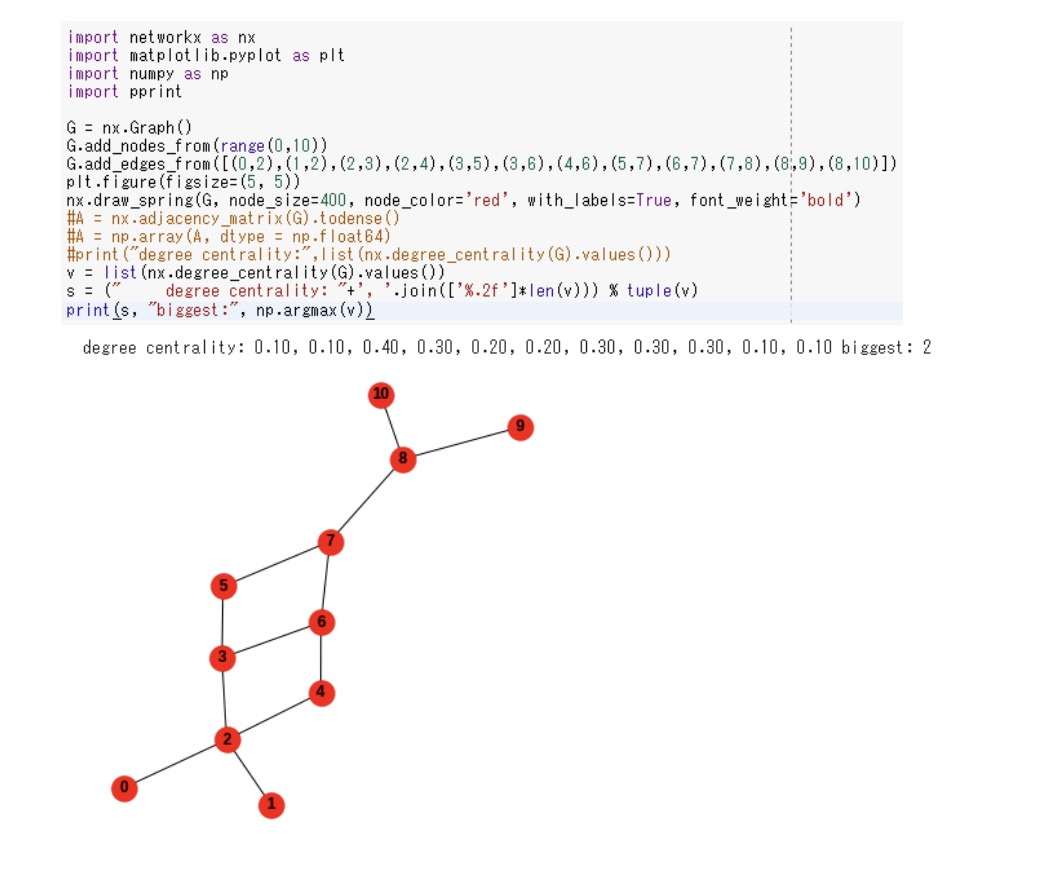
\includegraphics[scale=0.3]{quiz5_1.jpg}

\subsection*{Answer 1}

\begin{python}
import networkx as nx
import matplotlib.pyplot as plt
import numpy as np
import pprint

G = nx.Graph()
G.add_nodes_from(range(0,10))
G.add_edges_from([(0,2),(1,2),(2,3),(2,4),(3,5),(3,6),(4,6),(5,7),(6,7),(7,8),(8,9),(8,10)])
plt.figure(figsize=(5, 5))
nx.draw_spring(G, node_size=400, node_color='red', with_labels=True, font_weight='bold')
v = list(nx.degree_centrality(G).values())
s = ("     degree centrality: "+', '.join(['%.2f']*len(v))) % tuple(v)
print(s, "biggest:", np.argmax(v))
\end{python}

The result is:
\begin{python}
     degree centrality: 0.10, 0.10, 0.40, 0.30, 0.20, 0.20, 0.30, 0.30, 0.30, 0.10, 0.10 biggest: 2

\end{python}



\end{homeworkProblem}
\pagebreak

\begin{homeworkProblem}
2. Betweenness centrality

\subsection*{Answer2}

\begin{python}
import networkx as nx
import matplotlib.pyplot as plt
import numpy as np
import pprint

G = nx.Graph()
G.add_nodes_from(range(0,10))
G.add_edges_from([(0,2),(1,2),(2,3),(2,4),(3,5),(3,6),(4,6),(5,7),(6,7),(7,8),(8,9),(8,10)])
plt.figure(figsize=(5, 5))
nx.draw_spring(G, node_size=400, node_color='red', with_labels=True, font_weight='bold')
v = list(nx.betweenness_centrality(G).values())
s = ("     btweeenness centrality: "+', '.join(['%.2f']*len(v))) % tuple(v)
print(s, "biggest:", np.argmax(v))
\end{python}
The result is:
\begin{python}
     btweeenness centrality: 0.00, 0.00, 0.40, 0.30, 0.12, 0.13, 0.34, 0.49, 0.38, 0.00, 0.00 biggest: 7

\end{python}


\end{homeworkProblem}
\pagebreak




\begin{homeworkProblem}

3. Closeness centrality
% 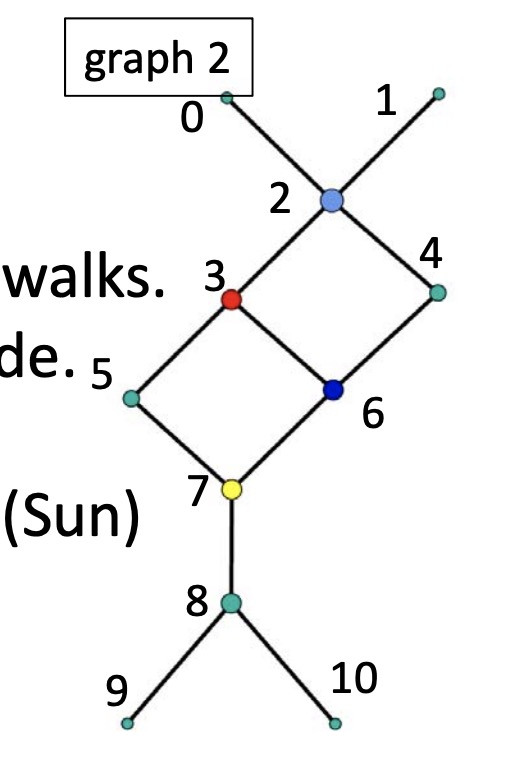
\includegraphics[scale=0.3]{quiz4_2.jpg}
\subsection*{Answer3}

\begin{python}
import networkx as nx
import matplotlib.pyplot as plt
import numpy as np
import pprint

G = nx.Graph()
G.add_nodes_from(range(0,10))
G.add_edges_from([(0,2),(1,2),(2,3),(2,4),(3,5),(3,6),(4,6),(5,7),(6,7),(7,8),(8,9),(8,10)])
plt.figure(figsize=(5, 5))
nx.draw_spring(G, node_size=400, node_color='red', with_labels=True, font_weight='bold')
v = list(nx.closeness_centrality(G).values())
s = ("     closeness centrality: "+', '.join(['%.2f']*len(v))) % tuple(v)
print(s, "biggest:", np.argmax(v))
\end{python}
The result is:
\begin{python}
     closeness centrality: 0.29, 0.29, 0.40, 0.45, 0.42, 0.43, 0.48, 0.45, 0.37, 0.28, 0.28 biggest: 6

\end{python}


\end{homeworkProblem}
\pagebreak

\begin{homeworkProblem}

4. Eigenvector centrality
\subsection*{Answer4}

\begin{python}
import networkx as nx
import matplotlib.pyplot as plt
import numpy as np
import pprint

G = nx.Graph()
G.add_nodes_from(range(0,10))
G.add_edges_from([(0,2),(1,2),(2,3),(2,4),(3,5),(3,6),(4,6),(5,7),(6,7),(7,8),(8,9),(8,10)])
plt.figure(figsize=(5, 5))
nx.draw_spring(G, node_size=400, node_color='red', with_labels=True, font_weight='bold')
v = list(nx.eigenvector_centrality(G).values())
s = ("     eigenvector centrality: "+', '.join(['%.2f']*len(v))) % tuple(v)
print(s, "biggest:", np.argmax(v))
\end{python}
The result is:
\begin{python}
     eigenvector centrality: 0.16, 0.16, 0.42, 0.45, 0.33, 0.31, 0.44, 0.36, 0.20, 0.07, 0.07 biggest: 3

\end{python}


\end{homeworkProblem}
\pagebreak


\begin{homeworkProblem}

5. PageRank
\subsection*{Answer5}

\begin{python}
import networkx as nx
import matplotlib.pyplot as plt
import numpy as np
import pprint

G = nx.Graph()
G.add_nodes_from(range(0,10))
G.add_edges_from([(0,2),(1,2),(2,3),(2,4),(3,5),(3,6),(4,6),(5,7),(6,7),(7,8),(8,9),(8,10)])
plt.figure(figsize=(5, 5))
nx.draw_spring(G, node_size=400, node_color='red', with_labels=True, font_weight='bold')
v = list(nx.pagerank(G).values())
s = ("     pagerank: "+', '.join(['%.2f']*len(v))) % tuple(v)
print(s, "biggest:", np.argmax(v))
\end{python}
The result is:
\begin{python}
     pagerank: 0.05, 0.05, 0.16, 0.11, 0.08, 0.08, 0.11, 0.12, 0.14, 0.05, 0.05 biggest: 2

\end{python}


\end{homeworkProblem}
\pagebreak

\begin{homeworkProblem}

6. Katz centrality
\subsection*{Answer6}

\begin{python}
import networkx as nx
import matplotlib.pyplot as plt
import numpy as np
import pprint

G = nx.Graph()
G.add_nodes_from(range(0,10))
G.add_edges_from([(0,2),(1,2),(2,3),(2,4),(3,5),(3,6),(4,6),(5,7),(6,7),(7,8),(8,9),(8,10)])
plt.figure(figsize=(5, 5))
nx.draw_spring(G, node_size=400, node_color='red', with_labels=True, font_weight='bold')
v = list(nx.katz_centrality(G).values())
s = ("     katz centrality: "+', '.join(['%.2f']*len(v))) % tuple(v)
print(s, "biggest:", np.argmax(v))
\end{python}
The result is:
\begin{python}
     katz centrality: 0.27, 0.27, 0.35, 0.33, 0.30, 0.30, 0.33, 0.33, 0.32, 0.26, 0.26 biggest: 2

\end{python}


\end{homeworkProblem}
\pagebreak

\end{document}
%
% Non sequential homework problems
%

% Jump to problem 18
